
\section{Background and Overview}

\label{sec:overview}

Our method is designed for boolean evaluations on arbitrary number of inputs primitives \cite{requicha1985boolean}. Primitives are triangular solid meshes free of self-intersecting. Geometry connectivity is also required as inputs. Even if there are topological deficiencies, our method still try to give acceptable answer. Our method is not sensitive to topological deficiencies which are not near the regions where primitives intersect.

In the following, we first discuss the causes of non-robustness of boolean methods. Then we analyze the cause of inefficiency of previous plane-based methods and discuss how to avoid these problems. Finally, we give an overview of the proposed method.


\subsection{Robustness of Boolean Methods}
\label{sec:paradigm}

The boolean evaluations on mesh primitives are, in essence, a process of face selection. Namely, given a boolean expression, the operation collect those faces that satisfy the expression to generate the final mesh. Whether a certain face $\bm{s}$ belong to the final mesh is determined by its inclusion labels and the boolean expression $f$:
\begin{equation}
\lambda_f(\bm{s}) = f(\boldsymbol{\Lambda}(\bm{s})) = f(\lambda_1(\bm{s}), \lambda_2(\bm{s}), \cdots, \lambda_n(\bm{s})),
\end{equation}
where $\lambda_i(\bm{s})$ is the inclusion label with respect to primitive $M_i$. Each label has four conditions: completely inside (\emph{in}), completely outside (\emph{out}), on the boundary with consistent normal vector (\emph{same}) or with opposite normal vector (\emph{oppo}). To compute $\lambda_f(\bm{s})$, the labels with respect to all of the primitives (as $\boldsymbol{\Lambda}(\bm{s})$) must be known.
The evaluation of boolean expression with inclusion labels are discussed in \cite{douze2015quickcsg,feito2013fast}. If and only if $\lambda_f(\bm{s})=same$, $\bm{s}$ is on the surface of the final mesh.

Unfortunately, not all of the input faces can be classified collectively. For some faces near the intersections, only parts of them belong to the final mesh. Therefore, an extra step before face classification is required to detect intersections between meshes. Then input meshes are tessellated according to these intersections to ensure that every face is completely inside, outside, or on the boundary of other input meshes.

Most of the existing boolean methods follow such two-step paradigm---intersection computation and face classification, as does our method. Non-robustness comes from three stages of such boolean methods. 1) The intersection between faces may not be exactly computed. 2) Face tessellation produces inconsistent topology. 3) The computation of the inclusion labels is not consistent with the location of the faces. These problems all come from the numerical errors during geometric computation. Therefore, if these three stages can be performed in exact ways, boolean evaluations are robust.

% \begin{figure}[t]
% \centering
% 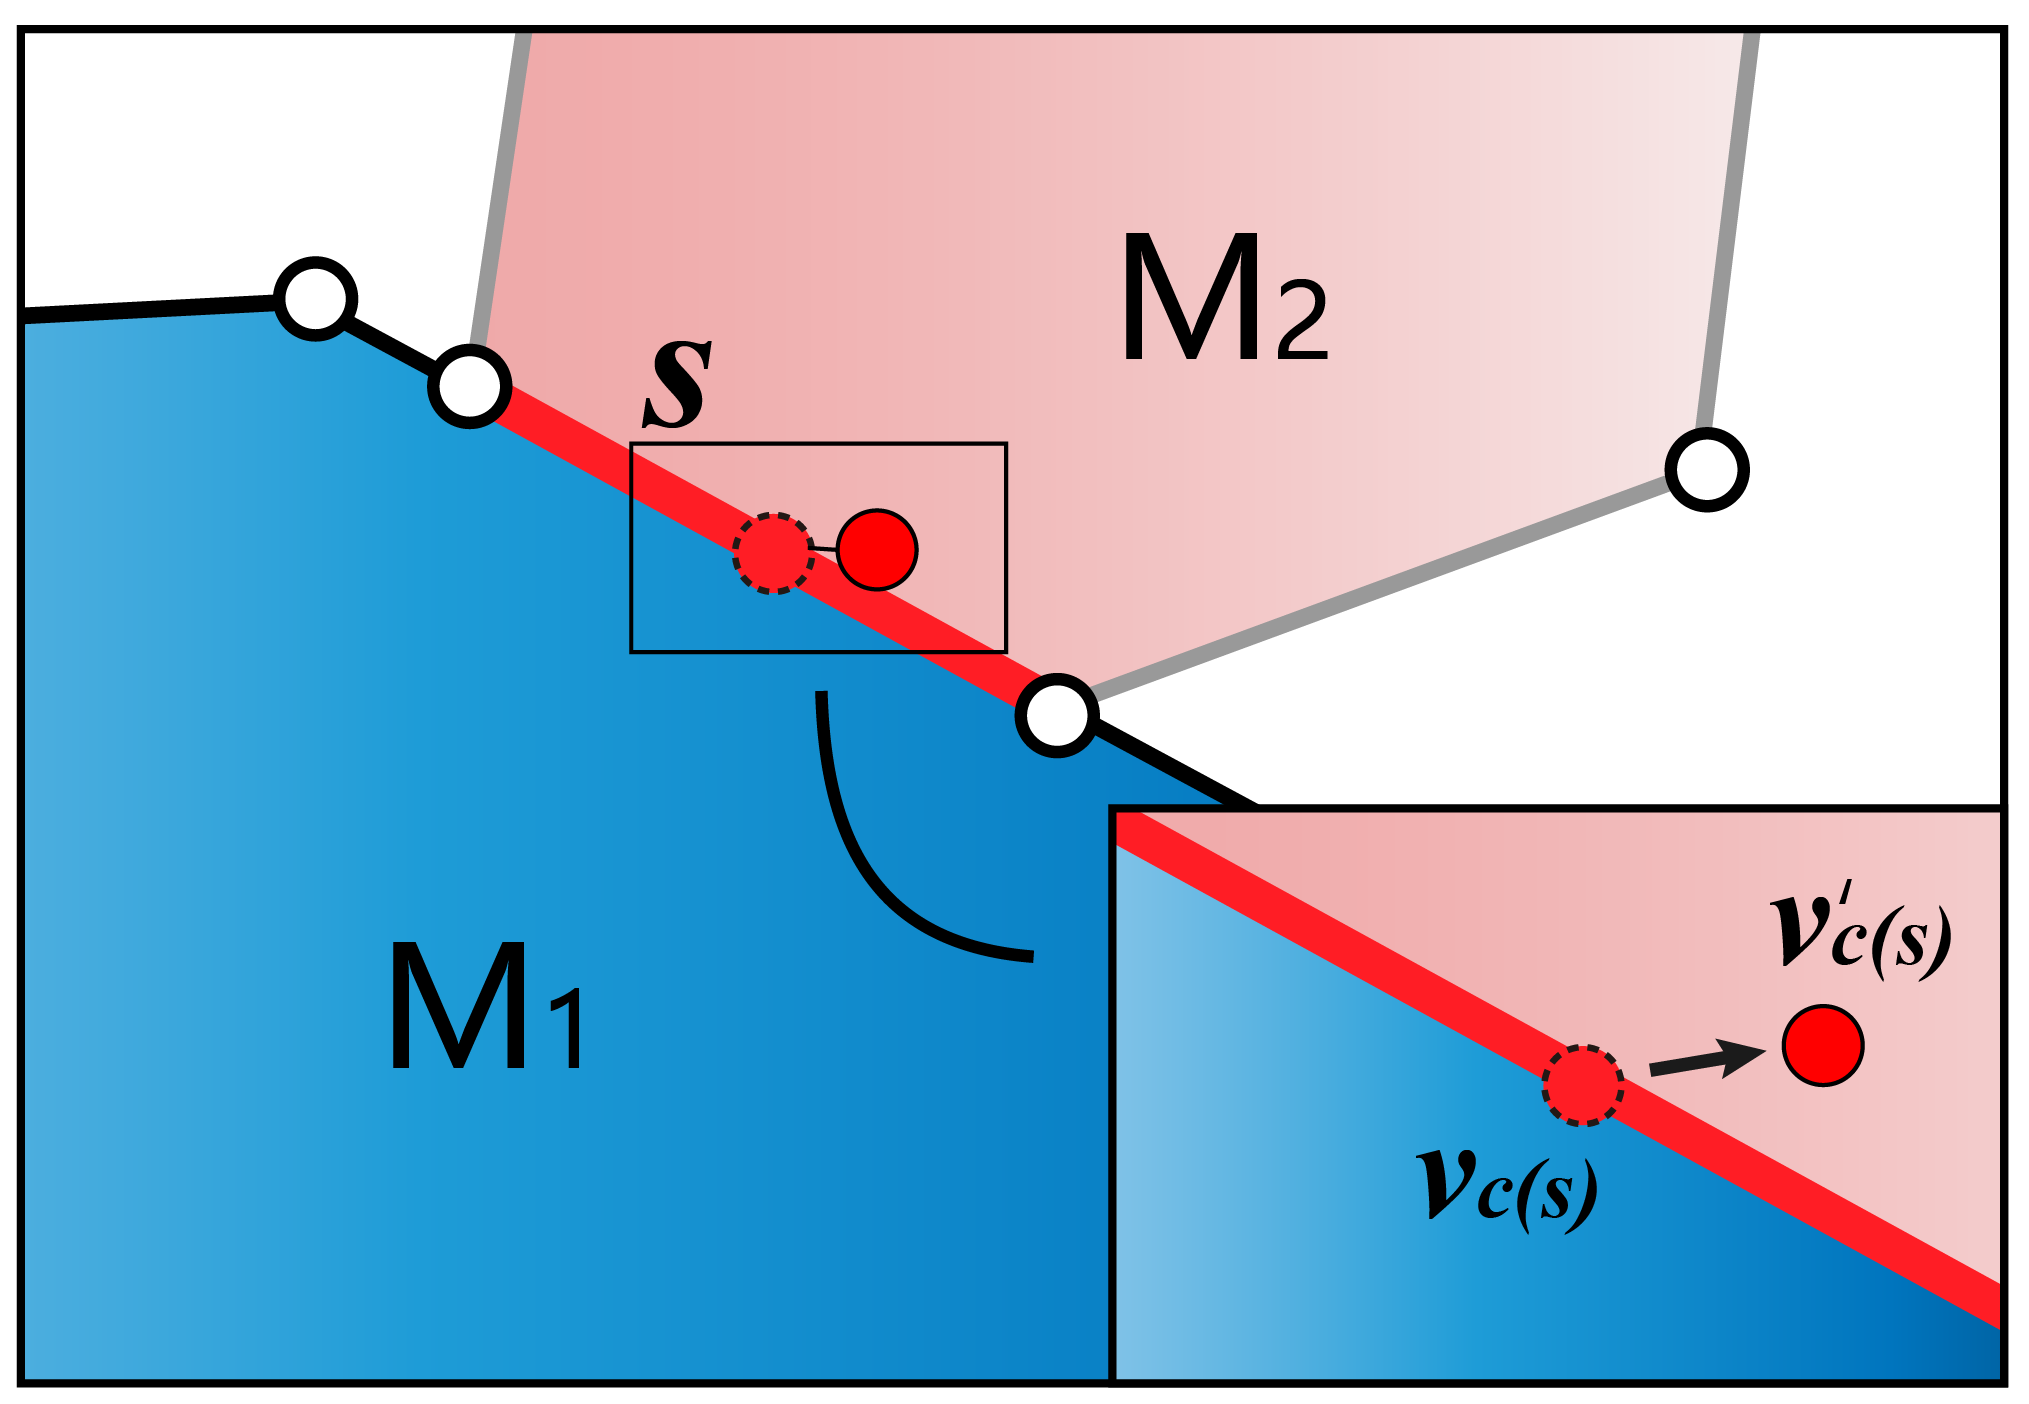
\includegraphics[width=2.2in]{boolean-01}
% \caption{In this 2D view, face $\bm{s}$ (the red line segment) of mesh $M_2$ is on the surface of mesh $M_1$. However, because the face barycenter $\bm{v}_{c(\bm{s})}$ is used to compute the labels, the coordinates of which contain round-off errors, the point could be moved to $\bm{v'}_{c(\bm{s})}$. Thus, $\bm{s}$ may be falsely classified as being outside of $M_1$.}
% \label{fig:falseclass}
% \end{figure}


\subsection{Plane-based booleans}
Comparing with applying exact arithmetic, using plane-based geometry \cite{campen2010exact} is more promising to produce efficient exact computations. Therefore, in our method, we use P-reps as the key to avoid numerical errors.

\label{sec:substrates}
\subsubsection{Plane-based representation}


\begin{wrapfigure}{r}[0in]{0in}
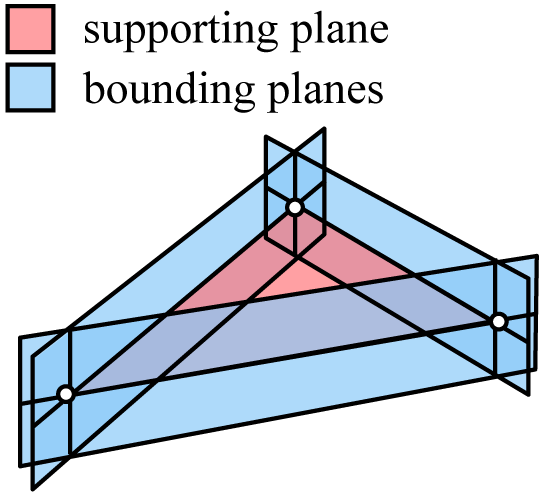
\includegraphics[width=1.5 in]{boolean-07}
\end{wrapfigure}

Using P-reps, each face $\bm{s}$ with $n$ edges is represented by a supporting plane $\bm{p}_{s,sp}$ on which the face lies, and a set bounding planes $\{\bm{p}_{s,b}^i \ \vert\  i = 0, 1,...,n-1\}$. Each edge line $\bm{e}_{\bm{s}}^i$ is represented by the intersection $\bm{p}_{s,sp} \cap \bm{p}_{s,b}^i$.
Vertex $\bm{v}_s^i$ is represented by the intersection of $\bm{p}_{s,sp}$ and two consecutive bounding planes. We use the method of Campen et al. \cite{campen2010exact} for the exact conversion of triangles to their P-reps. The exact plane-based predicates are sped up using numerical filtering techniques by Shewchuk \cite{shewchuk1997adaptive}.


Other commonly used notations in this paper are presented below. The normal of a plane $\bm{p}$ is denoted as $\bm{n}(\bm{p})$. A line $\bm{l}$ of P-reps can be represented by the intersection of two planes $(\bm{p}_l^0 \cap \bm{p}_l^1)$, hence, $\bm{l}\colon(\bm{p}_l^0 \cap \bm{p}_l^1)$. The positive direction of the line $\bm{l}$ is defined by $\bm{n}(\bm{p}_l^0) \times \bm{n}(\bm{p}_l^1)$.
A point $\bm{v}$ of P-reps can be represented by non-trivial plane triples $(\bm{p}_v^0 \cap \bm{p}_v^1 \cap \bm{p}_v^2)$, hence, $\bm{v}\colon(\bm{p}_v^0 \cap \bm{p}_v^1 \cap \bm{p}_v^2)$.

\subsubsection{Efficient embedding}

Under P-reps, vertex is represented with a much higher precision than under V-reps. A plane is represented by four parameters. Then a vertex takes twelve parameters under P-reps compared with only three parameters under V-reps. This makes geometric computations significantly slower under P-reps. Even though numerical filters can be applied to speed up, pure plane-based methods, such as \cite{sugihara1990solid,banerjee1996topologically}, are significant slower than vertex-based methods. On the other hand, a hybrid representation can bring both the efficiency of V-reps and the exactness of P-reps. And plane-based geometric computation should be avoided as much as possible to reduce computation cost.

BSP-based boolean algorithms are substantially based on planes, therefore are suitable to implement with P-reps \cite{bernstein2009fast,campen2010exact}. However, BSP merging is a pure plane-based algorithm. Also, BSP structure has additional two drawbacks which make it slow: a) BSP algorithms have high time complexity. b) BSP structure destroy geometry connectivity information, thus algorithms benefiting from connectivity require extra effort to reconstruct connectivity. Therefore, as an exact but not efficient representation, BSP should not substitute V-reps in total, but can serve as a compliment of V-reps to help plane-based geometric computation. Also, BSP structure has to be localized to minimize its size.

In our method, we use V-reps for coarse tests and fast connectivity queries and P-reps for exact predicates. The framework of our method is based on \cite{ogayar2015deferred}, which is a vertex-based method. Plane-based algorithms are embedded into the processing. This embedding is not a simple plane-based implementation of vertex-based algorithms. We develop three efficient algorithms which is optimized under P-reps: triangle-triangle intersection tests, triangle tessellation and polygon classification. These three algorithms are corresponding to the three sources of non-robustness discussed in \S\ref{sec:paradigm}. The major difficulty is to guarantee the efficiency and exactness simultaneously. For this purpose, we avoid any computation under high precision, which means our method is designed to be implemented using only common double-precision floating-point arithmetic.

\subsubsection{Mapping to three diemensions}

Many vertex-based algorithms, such as 2D triangulation and face classification, is hard to implement under P-reps because they requires projection from three dimensions to planes or lines.  Projections are performed on vertex coordinates which are absent under P-reps. Since plane-based predicates \cite{bernstein2009fast,banerjee1996topologically} are usually performed under three dimensions, we have to find the equivalent three dimensional problem, whose projection to low dimension is the problem we want to compute. In the following, we discuss three such plane-based algorithms used in our method.

\vspace{0.5em}
\noindent \textbf{Point-line orientation}

\noindent Within the plane $\bm{p}_0$, the point-line orientation is computed by the line parameters and point coordinates under V-reps. Under P-reps, we map this problem to point-plane orientation by picking a plane $\bm{p_l}$ which satisfy three requirements: 1) the line is in $\bm{p_l}$; 2) $\bm{p_l}$ is not parallel with $\bm{p}_0$; 3) $\bm{n}(\bm{p}_0) \times \bm{n}(\bm{p_l})$ has the same orientation as the line.

\vspace{0.5em}
\noindent \textbf{Linear ordering of points}

\begin{figure}
  \centering
  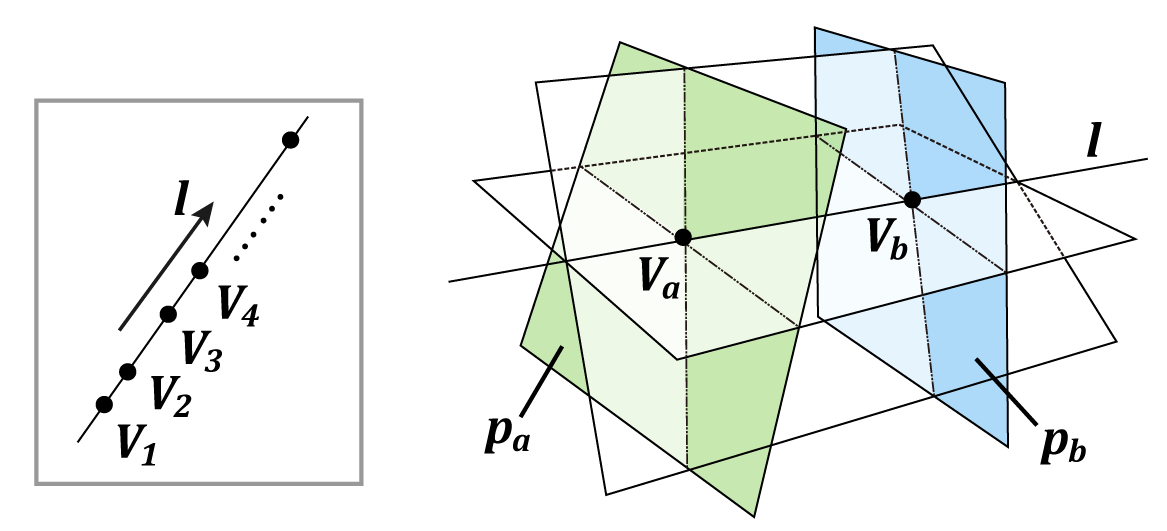
\includegraphics[width=3.5in]{boolean-09}\\
  \caption{Geometric configuration of the linear ordering of points. Points $\bm{v}_a$ and $\bm{v}_b$ are both on line $\bm{l}_{ab}$. We convert this problem into the plane ordering of $\bm{p}_a$ and $\bm{p}_b$ along $\bm{l}_{ab}$.}\label{fig:twopointoneline}
\end{figure}

\noindent Given a line $\bm{l}$ with two points on it, $\bm{v}_a\colon(\bm{p}_a^0\cap\bm{p}_a^1\cap\bm{p}_a^2)$, and $\bm{v}_b\colon(\bm{p}_b^0\cap\bm{p}_b^1\cap\bm{p}_b^2)$, we need to determine the linear order of the two points along $\bm{l}$ (see Fig. \ref{fig:twopointoneline}).
To solve this problem, we choose one plane that is not parallel with $\bm{l}$ from the P-rep of each point, then convert this problem into one of determining the linear order of planes, which can be solved using the method of Banerjee et al. \cite{banerjee1996topologically}. The chosen planes should have the same orientation with respect to $\bm{l}$ (the dot product between the plane normal and $\bm{l}$ must be positive), and unqualified planes need to be flipped.


\begin{wrapfigure}{r}[0in]{0in}
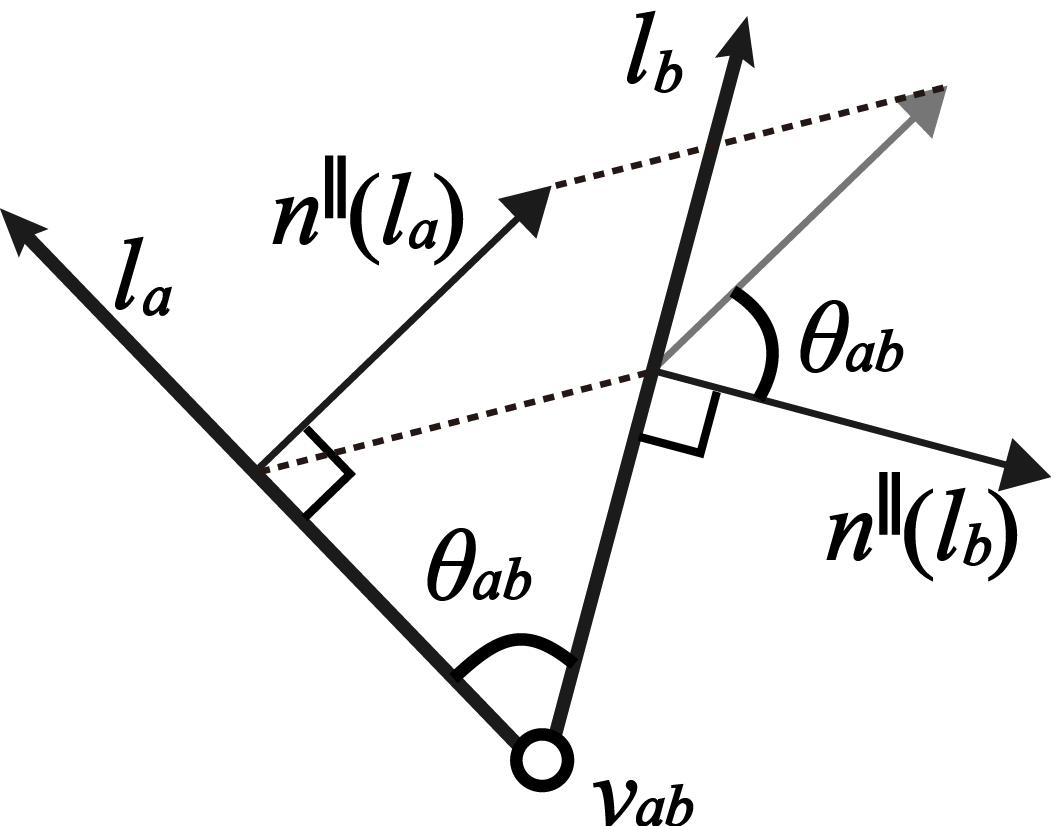
\includegraphics[width=1.5 in]{boolean-02}
\end{wrapfigure}
\vspace{0.5em}
\noindent \textbf{Circular ordering of lines}~~~~

\noindent During face tessellation, we need to know which intersections are neighbors (see Fig. \ref{fig:circularorder}). This requires circular ordering of directed lines around a vertex. The Lines can be sorted in a divide-and-conquer way, based on the relative order of each pair of lines. Thus, this problem is converted to one where, given two lines $\bm{l}_a$ and $\bm{l}_b$ in a plane $\bm{p}_0$, circular order of the two lines needs to be computed.
We can compute the order by the sign of $\sin{\theta_{ab}}$, where $\theta_{ab}\in(-\pi,\pi)$ is the angle from $\bm{l}_a$ to $\bm{l}_b$ in the top-view of $\bm{p}_0$.

We know the sign of $\sin{\theta_{ab}}$ is the same as the sign of $\bm{n}(\bm{p}_0) \cdot (\bm{l}_a\times\bm{l}_b)$. However, directly computing this equation requires extra precision to explicitly compute $\bm{l}_a$ and $\bm{l}_b$. Fortunately, we found a efficient solution which only needs to compute the sign of a 3$\times$3 determinants, whose elements are all floating-point numbers.

\begin{theorem}
  \label{theorem1}
  Given two directed lines $\bm{l}_a\colon(\bm{p}_0\cap\bm{p}_a)$ and $\bm{l}_b\colon(\bm{p}_0\cap\bm{p}_b)$ within plane $\bm{p}_0$, the following relation always stands:
  \begin{equation}
    sign(\sin{\theta_{ab}})=  sign(\bm{n}(\bm{p}_0)\cdot(\bm{n}(\bm{p}_a) \times \bm{n}(\bm{p}_b)))
  \end{equation}
\end{theorem}

\begin{proof}
 First, $\bm{n}(\bm{p}_a)$ and $\bm{n}(\bm{p}_b)$ are orthogonally decomposed along $\bm{n}(\bm{p}_0)$:
 \begin{equation}
 \begin{split}
   &\bm{n}(\bm{p}_a)= \bm{n}^\parallel(\bm{p}_a) + \bm{n}^\perp(\bm{p}_a)\\
   &\bm{n}(\bm{p}_b)= \bm{n}^\parallel(\bm{p}_b) + \bm{n}^\perp(\bm{p}_b),
 \end{split}
 \end{equation}
 where the superscript $\parallel$ refers to the component parallel with $\bm{p}_0$ and $\perp$ means the component orthogonal to $\bm{p}_0$. Since $\bm{n}(\bm{p}_0)$ is orthogonal with $\bm{p}_0$, we get:
 \begin{equation}
   \label{eq:circ1}
   \bm{n}(\bm{p}_0) \cdot (\bm{n}(\bm{p}_a) \times \bm{n}(\bm{p}_b)) = \bm{n}(\bm{p}_0) \cdot (\bm{n}^\parallel(\bm{p}_a) \times \bm{n}^\parallel(\bm{p}_b)).
 \end{equation}
 On the other hand, the angle between $\bm{n}^\parallel(\bm{p}_a)$ and $\bm{n}^\parallel(\bm{p}_b)$ is exactly $\theta_{ab}$. Therefore,
 \begin{equation}
   \label{eq:circ2}
   sign(\sin{\theta_{ab}})=  sign(\bm{n}(\bm{p}_0) \cdot (\bm{n}^\parallel(\bm{p}_a) \times \bm{n}^\parallel(\bm{p}_b))).
 \end{equation}
 By (\ref{eq:circ1}) and (\ref{eq:circ2}), the theorem is proved.
\end{proof}

\begin{figure}[t]
\centering
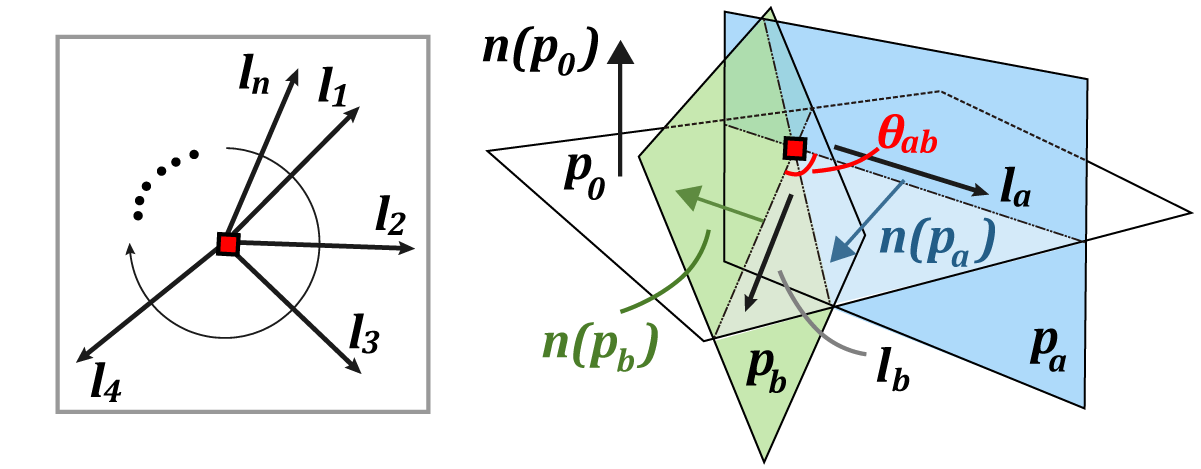
\includegraphics[width=3.5in]{boolean-08}
\caption{Geometric configuration of the circular ordering of lines. $\bm{l}_a\colon(\bm{p}_0 \cap \bm{p}_a)$ and $\bm{l}_b\colon(\bm{p}_0 \cap \bm{p}_b)$ are within plane $\bm{p}_0$.}
%Geometric configuration of the circular ordering of lines. la:
\label{fig:circularorder}
\end{figure}

\subsection{Method Overview}

Before going into details, we give an overview of our method. While the framework is similar to vertex-based boolean method, we address the major differences in each stage and briefly explain why these differences are necessary.

\subsubsection{Intersection computation}

We compute the intersections between pairs of triangles. The triangle-triangle intersection algorithm is largely based on M\"{o}ller's algorithm \cite{moller1997fast}. However, the conventional vertex-based implementation of M\"{o}ller's algorithm introduces numerical errors. Our plane-based intersection algorithm implicitly represents intersections using planes to avoid errors. In addition, we carefully deal with all of the degenerate situations, including point intersections, edge intersections, and coplanar intersections. Furthermore, octree is used to speed up the process. Details are provided in \S\ref{section:isect}.

\subsubsection{Deferred tessellation}

Once all of the intersections between triangles are determined, input meshes are subdivided, so that all intersections occurs on edges and vertices. In many existing methods (e.g., \cite{ogayar2015deferred,zhou2016mesh}), 2D constrained Delaunay triangulation (CDT) \cite{chew1989constrained,de1992line} is used to implement this stage. In our method, intersections are represented by planes. Therefore, projection is not allowed and the 2D CDT has to be mapped to an equivalent 3D problem. However, a 2D CDT needs to construct edges between arbitrary pair of vertices, whose equivalent 3D operation is to construct new planes. The newly constructed planes have to contain arbitrary pair of vertices, thus require extra precision to represent.

To avoid this problem, we choose to tessellate in a more conservative way that do not add any new edges. As a consequence, the subdivided faces are no more triangles but polygons. We first perform intersection refinement to resolve intersections between intersections. We then construct a graph-like structure, called \emph{tess-graph}, to guide the exact tessellation of each face. Details are given in \S\ref{sec:tessellation}.

\subsubsection{Face classification}

The purpose of this step is to collect faces that pass the boolean expression from the tessellated meshes to generate the final mesh. However, literally computing the inclusion label vector of each face is unacceptably slow for large CSGs. We utilize the connectivity information to propagate inclusion labels in a flood-filling manner. Typically, the seed face label is deduced by the label of a point on that face. However, the computation of point label can be incorrect without exact arithmetic. We exactly computed face label by a local BSP constructed according to the faces of neighborhoods. Our algorithm does not requires exact arithmetic. Also, the constructed BSP is typically small, which resulting in good performance. Details are given in \S\ref{sec:classification}.
